\section{Mapeamento}
   Vamos começar a entender o que é uma estrutura algébrica como introdução. Tome um conjunto $S$ e incorpore esse conjunto com uma estrutura algébrica assumindo que nós podemos combinar, de várias formas (geralmente em duas), os elementos desse conjunto $S$ para obter os elementos desse conjunto $S$. Isso que estamos fazendo aqui é combinar elementos do conjunto $S$, denominado de \textit{operações em $S$}. Uma coisa importante para saber agora é que o comportamento dessas operações em $S$ podem ser condicionadas impondo certos axiomas, alterando a natureza de $S$. Os axiomas definem a particularidade da estrutura em $S$. Se eu quiser pegar uma coleção de axiomas e testá-los na tentativa de definir novas estruturas seria algo possível. Repare nas palavras "testá-los" e "tentativa". Uma estrutura algébrica depende fortemente de \textbf{consistência} entre sua coleção de axiomas. Mesmo assim ainda não seria suficiente para evitar criar um sistema estranho. Daqui em diante trataremos os axiomas como regras que são validadas dentro de um sistema algébrico, não como verdades evidentes como é popularmente entendido.
   \subsection{Função Geral}
      Sendo $X$ um conjunto de todos os objetos em venda num mercado e $Y$ ser o conjunto de todos os números reais. Definimos $f:X \to Y$ como $f(x) = \textrm{preço de x}$. Isso é um exemplo de mapeamento de $X$ para $Y$.
      Um exemplo de função: Sendo $X$ um conjunto não vazio e definindo $i:X \to X$ como $i(x) = x$ para qualquer $x \in X$. Chamamos essa função, onde temos $X$ para $X$, de função identidade.\newline
      Um mapeamento é uma função geral que associa um elemento de uma origem a um elemento \textbf{único} do destino. Chamaremos $f$ como um mapeamento de $X$ para $Y$ por $f:X \to Y$ e, para $y \in Y$, $y = f(x)$; $y$ é \textit{imagem} de $x$ sob $f$.
      Assim, uma função é um mapa de um domínio $D$ para um contradomínio $CD$ tal que cada elemento de $D$ tem pelo menos uma imagem em $CD$.

      \begin{definition}
         Se $g:X \to Y$ e $f:Y \to Z$, então a \emph{composição}, denotada por $f \circ g$, é o mapameanto $f \circ g: X \to Z$ definido por $(f \circ g)(x) = f(g(x))$ para todo $x \in X$.
      \end{definition}
      \begin{lemma}\label{comp-assoc}
      Se $h:X \to Y, g:Y \to Z$\ e\ $f:Z \to W$, então $f\circ (g\circ h) = (f \circ g)\circ h.$
      \begin{proof}
         Temos que verificar que se esses dois mapeamento são iguais eles devem fazer a mesma coisa para qualquer elemento.\\
         $\forall x \in X, (f\circ(g\circ h))(x) = ((f \circ g)\circ h)(x).$ A aplicação da definição de composição segue $$(f\circ (g\circ h))(x)=f((g\circ h)(x))=f(g(h(x)))$$ $$((f\circ g)\circ h)(x)=(f\circ g)(h(x))=f(g(h(x))),$$ $$(f\circ (g \circ h))(x)=((f \circ g)\circ h)(x), \forall x \in X.$$
         Consequentemente, por definição, $f \circ (g \circ h) = (f\circ g) \circ h.$
      \end{proof}
      \end{lemma}

      \subsubsection{Funções Lineares}
         Uma das mais importantes classes de funções. Considere o conjunto $$ \R_{m}^{n} = \left\{
         \begin{bmatrix}
            a_{11} & \cdots & a_{1n} \\
            \vdots &  & \vdots \\
            a_{m1} & \cdots & a_{mn}
         \end{bmatrix}
         \mid a_{ij} \in \R \right\}.$$
         Em particular, $\R_{2}^{1}$ é o conjunto dos vetores coluna bidimensionais $$\hat{v} = 
         \begin{bmatrix}
            v_{1} \\
            v_{2}
         \end{bmatrix}; v_{1}, v_{2} \in \R.$$
         Cada matriz real quadrada de ordem $2$ resulta em uma função linear $$ L_{A}:\R_{2}^{1} \to \R_{2}^{1}; 
         \begin{bmatrix}
            v_{1} \\
            v_{2}
         \end{bmatrix}
         \mapsto 
         \begin{bmatrix}
            a_{11}v_{1} + a_{12}v_{2} \\
            a_{21}v_{1} + a_{22}v_{2}
         \end{bmatrix}$$
         ou $$L_{A}\left(\hat{v}\right) = A\hat{v}.$$
         Claro que $$L_{A} 
         \begin{bmatrix}
            1 \\
            0
         \end{bmatrix} =
         \begin{bmatrix}
            a_{11} \\
            a_{21}
         \end{bmatrix} \quad \textrm{e} \quad L_{A} 
         \begin{bmatrix}
            0 \\
            1
         \end{bmatrix} =
         \begin{bmatrix}
            a_{12} \\
            a_{22}
         \end{bmatrix},$$
         isto é, a função linear $L_{A}$ determina a matriz $A$. Seja $B$ uma matriz quadrada de ordem $2$ com uma função linear correspondente $L_{B}: \hat{v}\mapsto B\hat{v}$, $BA$ é definida por
         $$\begin{bmatrix}
            b_{11} & b_{12} \\
            b_{21} & b_{22}
         \end{bmatrix}
         \begin{bmatrix}
            a_{11} & a_{12} \\
            a_{21} & a_{22}
         \end{bmatrix} = 
         \begin{bmatrix}
            b_{11}a_{11} + b_{12}a_{21} + b_{12}a_{22} \\
            b_{21}a_{11} + b_{22}a_{21} + b_{22}a_{22}
         \end{bmatrix}.$$
         A equação $L_{BA} (\hat{v}) = L_{B} \circ L_{A} (\hat{v})$ é verdadeira para todo $\hat{v}$ em $\R_{2}^{1}$.\\
         A multiplicação de matrizes acompanha a composição das funções lineares correspondentes. Em particular, a associatividade da multiplicação de matriz é uma consequência direta da associatividade da composição de funções (\textbf{Lema} \ref{comp-assoc}).

      \subsubsection{Semigrupos de Funções}
         Um mapa (ou função) $f: X \to X$ de $X$ para ele mesmo é muitas vezes dito como um \emph{autom-mapa} do conjunto $X$. Nesse contexto, o conjunto algumas vezes é chamado de \emph{conjunto base} para a função $f: X \to X$.
         \begin{definition}
            Um conjunto $S$ de funções $f: X \to X$ com o domínio $X$ e contradomínio $X$ é dito ser um semigrupo de funções no conjunto base $X$ se $$f\quad \textrm{e}\quad g\quad \textrm{em}\quad S\quad \textrm{implica}\quad g \circ f\quad \textrm{em}\quad S. $$
            Nesse caso, $S$ está fechado sob a composição (composta).

            Se $f$ é um elemento de um semigrupo $S$ de funções, as exponenciais $f^n$ para $n$ inteiros positivos são definidas recursivamente por $f^{1} = f$ e $f^{n+1} = f^n \circ f.$

            Alguns exemplos de semigrupos de funções são:
            \begin{exmp}[Auto-mapas]
               Para um conjunto base $X$, defina $X^X$ como o conjunto de todas as funções de $X$ para $X$. Então $X^X$ forma um semigrupo de funções em $X$.
            \end{exmp}
         \end{definition}
         \begin{exmp}[Funções constantes]
            Seja $X$ um conjunto e $Y$ um subconjunto de $X$. Para cada elemento $y$ de $Y$, define uma função constante
            \begin{alignat}{2}
               c_{y}:\ &X \to X \nonumber\\
               &x\ \mapsto\ y.
               \nonumber
            \end{alignat}
            Ainda temos que para cada elemento $x$ de $X$, $y \in X$ e $z$ no subconjunto $Y$
            $$c_{z} \circ c_{y}(x) = c_{z}\left(c_{y}(x)\right) = c_{z}(y) = z = c_{z}(x),$$
            ou seja, $c_{z} \circ c_{y} = c_{z}$. Assim o conjunto $$C_{Y} = \left\{c_{y}\mid y \in Y\right\}$$ forma um semigrupo de funções em $X$.
         \end{exmp}
         \begin{definition}[Função identidade]
            Para qualquer conjunto $X$, a função identidade $id_{X}$ é definida por
            \begin{alignat}{2}
               id_{X}:\ &X \to X \nonumber\\
               &x\ \mapsto\ x.
               \nonumber
            \end{alignat}
            Para conjuntos $X$, $Y$ e $f: X \to Y$, temos
            $$id_{Y}\circ f = f = f \circ id_{X}.$$
         \end{definition}
         \begin{definition}[Monoide de Funções]
            Um conjunto $S$ de auto-mapas em um conjunto base $X$ é dito ser um Monoide de funções em $X$ se formar um semigrupo e se a função identidade $id_{X}$ é um elemento de $S$.
         \end{definition}
         Um exemplo trivial de um Monoide de função é o conjunto $X^X$ em $X$.
         \begin{exmp}
            Pelas funções lineares o conjunto $L\left(2,\R\right)$ das funções lineares de $\R_{2}^{1}$ para ele mesmo forma um semigrupo de funções em $\R_{2}^{1}$. Agora para a matriz identidade
            $$I_{2} = \begin{bmatrix}
               1 & 0\\
               0 & 1
            \end{bmatrix}
            $$
            a função linear $L_{I_{2}}$ é a função identidade $id_{\R_{2}^{1}}$, então $L\left(2,\R\right)$ forma um Monoide de funções em $\R_{2}^{1}.$
         \end{exmp}

      \subsubsection{Injetividade e sobrejetividade}
         Um mapeamento (a função $f$) $f: X \to Y$ precisa associar um unico valor da função $f(x)$ no contradomínio $Y$ para cada argumento $x$ do domínio $X$. Por outro lado, pode acontecer que argumento diferentes sejam associados ao mesmo valor $f(x)$. O caso trivial que serve de exemplo é a função dos quadrados $sq: \Z \to \N$ onde poderiamos ter $$sq(-5) = (-5)^{2} = 25 = 5^{2} = sq(5).$$
         \begin{definition}[Função Injetiva]
               Uma função $f: X \to Y$ é dita ser injetiva, ou \emph{um para um}, se $$f(x) = f(x') \implies x = x'$$
            para todos elementos $x$ e $x'$ do domínio $S$.
            Em essência, a equação $f(s) = t$ precisa ter uma única solução $x$ em $X$ para cada elemento $y$ para a imagem de $f$. É imediato que qualquer função com um domínio vazio seja injetiva. Diferente da função $sq: \Z \to N$, a função $sqn: \N \to \N; n \mapsto n^{2}$ é injetiva.
         \end{definition}
         \begin{stat}[Retração de funções injetivas]
            Deixe $f: X \to Y$ injetiva, com o domínio não vazio. Então existe uma função $$r: Y \to X$$
            tal que $$r \circ f = id_{X}.$$
            \begin{proof}
               Escolha um elemento $x_{0}$ de $X$. Para um elemento $y$ do contradomínio que
               não está na imagem $f(X)$, defina $r(y) = x_{0}$. Agora considere um elemento $y$ da imagem de $f(X)$. Pela definição de imagem, a equação $f(x) = y$ tem um solução. Como $f$ é injetiva, a solução é única. 
               
               Defina $r(y)$ como este único elemento de solução $x_{y}$. 
               
               Obtemos uma função $r: Y \to X$. Agora $r \circ f: X \to X$. Então para cada elemento $x$ de $X$, temos $$r\circ f(x) = r \left(f(x)\right) = x_{f(x)} = x = id_{X}(x),$$ que verifica $r \circ f = id_{X}.$
            \end{proof}
         \end{stat}
         
         \begin{definition}[Retração]
            Um mapeamento $r: Y \to X$ é cahamado de uma retração de uma função $f: X \to Y$ se $r\circ f = id_{X}.$
         \end{definition}
         \begin{stat}[Funções com retrações são injetivas]
            Se uma função $f: X \to Y$ possui uma retração (volta), então ela é injetiva.
         \end{stat}
         \begin{proof}
            Deixe $r: Y \to X$ ser uma retração para $f$. Então $$f(x) = f(x') \implies x=r\circ f(x) = r\circ f(x') = x'$$ para $x,x'$ em $X$.
         \end{proof}
         A proprosição anterior mostra que cada injeção com domínio não vazio tem uma retração. Note que um injeção $f$ pode ter muitas retrações, por causa da escolha arbitrária do elemento $x_{0}$ na prova da existência da retração. Também, note que a função identidade $id_{\varnothing}$ no conjunto vazio possui sua própria retração.

         \begin{definition}[Função Sobrejetiva]
            Uma função $f: X \to Y$ é dita ser sobrejetiva se o contradomínio e imagem coincidem: $Y = f(X)$.
         \end{definition}
         Maneiras para dizer que um mapeamento $f: X \to Y$ é sobrejetivo:
         $$f(X) = \{f(x) \in Y \mid x \in X\}$$
         $$f(X) = Y.$$
         Ainda, a imagem inversa $$f^{-1}\{y\} = \left\{x \in X \mid f(x) = y\right\}$$
         necessita ser não vazia para cada elemento $y$ de $Y$. Perceba que a única função sobrejetiva com um domínio vazio é a função identidade $id_{\varnothing}$ no conjunto vazio.

         Um exemplo trivial de uma função sobrejetiva seria a função do valor absoluto $abs: \Z \to \N; n \mapsto \mid n \mid$
         \begin{stat}[Seções de funções sobrejetivas]
            Deixe $f: X \to Y$ ser sobrejetiva. Então existe uma função $$s: Y \to X$$ tal que $$f \circ s = id_{y}.$$
         \end{stat}
         \begin{definition}[Seções]
            Uma função $s: Y \to X$ é chamada de seção de uma função $f: X \to Y$ se $f \circ s = id_{Y}.$
         \end{definition}
         \begin{stat}[Funções com seções são sobrejetivas]
            Se uma função $f: X \to Y$ tem uma seção, então ela é sobrejtiva.
            \begin{proof}
               Deixe $s: Y\to X$ ser uma seção para $f$. Então $$f\left(s(y)\right) = f\circ s(y) = id_{Y} = y$$
               para cada elemento $y$ de $Y$.
            \end{proof}
         \end{stat}
         Cada sobrejeção tem uma seção. Note que uma sobrejeção $f$ pode ter muitas seções.

      \subsubsection{Isomorfismo}
         \begin{definition}[Isomorfismo de conjuntos]
            A função $f:X \to Y$ é bijetivo se $f$ é injetivo e sobrejetivo.
         \end{definition}
         A utilização do mapeamento começa a se expandir quando entramos em composições de mapeamentos. Situa-se dois mapeamentos $g:X \to Y$ e $f:Y \to Z$. Queremos fazer com que os elementos de $X$ sejam conduzidos ao conjunto $Z$. Com efeito, $g(x) \in Y$, sendo $f:Y \to Z$, tem-se a disponibilidade de $f(g(x)) \in Z$. Assim, $(f\circ g):X \to Z$. Então, há o mapeamento de $X$ para $Z$.
         \begin{lemma}
            Se $f:X \to Y$ é uma bijeção, então $f\circ f^{-1} = id_{Y}$ e $f^{-1} \circ f=id_{X}$, onde $id_{X}$ e $id_{Y}$ são as identidades dos mapeamentos de $X$ e de $Y$, respectivamente.
            \begin{proof}
               Primeiramente, temos $(f\circ f^{-1})(y)=f(f^{-1}(y))$. Pela definição, $f^{-1}$ é o elemento $x_{0}\in X$ tal que $y=f(x_{0})$. Então $f(f^{-1}(y))=f(x_{0})=y$. Ora, isso significa que $(f\circ f^{-1})(y) = y$, validando a identidade deste mapeamento em $Y$.
            \end{proof}
         \end{lemma}
         Para $f^{-1}\circ f = id_{X}$ funciona analogamento como para $id_{Y}$
         \begin{definition}
            Para uma função $f: X \to Y$, uma função $g: Y \to X$ satisfazendo $g \circ f = id_{x}$ e $f \circ g = id_{Y}$ é chamado de inversa de $f$.
         \end{definition}
         Se existe um isomorfismo $f: X \to Y$ de um conjunto $X$ para um conjunto $Y$, podemos escrever $$X \cong Y$$ e dizer que os conjunto $X$ e $Y$ são isomorfico. Nesse caso $Y \cong X$, em virtude do isomorfismo $f^{-1}$.\\
         A ténica padrão para mostrar que dois conjuntos $X$ e $Y$ são isomorficos exibir duas funções mutuamente inversas $f: X \to Y$ e $g: Y \to X$.
         \begin{exmp}
            Para cada númera natural $n$, considere o conjunto finito $$N = \{0,1,2, ..., n -1\}$$
            dos números naturais menos do que $n$. Note que o conjunto $N$ tem $n$ elementos. Em particular, $\widehat{0}$ é o conjunto vazio. Agora, se um conjunto finito $X$ tem $n$ elementos, digamos $X = \{x_{0},x_{1},...,x_{n-1}\}$, então existe uma bijeção
            \begin{alignat}{2}
               K:\ &N \to X \nonumber\\
               &i\ \mapsto\ x_{i}.
               \nonumber
            \end{alignat}
         \end{exmp}
         De fato, um conjunto $X$ tem $n$ elementos se, e somente se existe uma bijeção $K: N\to X$. Nós podemos dizer que $K$ \emph{conta}  os elementos de $X$. O número dos elemetnos em um conjunto finito $X$ é chamado de \emph{tamanho} ou \emph{ordem} de $X$. É escrito como $\mid X\mid$. Dois conjunto são isomorficos se e somente se $\mid X\mid = \mid Y\mid$.

      \subsubsection{Grupos de permutações}
         \begin{definition}
            Deixe $X$ ser um conjunto.
            \begin{enumerate}[i.]
               \item Uma função bijetiva $f: X \to X$ é chamada de uma permutação do conjunto $X$.
               \item Um conjunto $G$ de permutações em $X$ é dito ser um grupo de permutações de $X$ ou uma permutação no conjunto $X$ se $G$ é um Monoide de funções satisfazendo a seguinte propriedade $$f \in G \implies f^{-1} \in G$$, também conhecida como \emph{fechada sob a inversão}.
            \end{enumerate}
         \end{definition}

   \subsection{Equivalência}
      Ao estudarmos uma estrutura precisamos filtrar o que não é relevante para o estudo dela. A equivalência é este filtro. Um exemplo inicial de sua necessidade surge no conceito de número. O que significa o número 3? Um conjunto $X$ tem 3 elementos se e somente se existe um isomorfismo de conjunto $$f: \{1,2,3\} \to X$$
      contando os elementos de $X$ como $f(1), f(2)$ e $f(3)$. A função $f$ tem que ser injetiva, de modo que nenhum elemento de $X$ seja contado duas vezes. A função $f$ tem que ser sobrejetiva, para garantir que cada elemento de $X$ seja contado.

      O único problema aqui é a circularidade. Para caracterizar o número 3, nós usamos esse número no domínio da função acima. Para escapar da circularidade nós podemos decidir considerar dois conjuntos como equivalentes para própositos de contagem sempre que eles forem isomórficos. O número 3 surge então como a propriedade que é comum a cada um dos conjuntos que são isomórficos a algum dado conjunto de 3 elementos (por exemplo $\{1,2,3\})$ ou $\{\varnothing , \{\varnothing\} , \{\{\varnothing\}\}\}$). Os detalhes particulares dos elementos nos conjuntos não são relevantes para o problema da contagem, Eles são filtrados pela equivalência.

      \subsubsection{Núcleo e relações de equivalência}
         Considere a função dos quadrados $sq: \Z \to \Z; n\mapsto n^{2}$. Para dois inteiros $n_{1}$ e $n_{2}$, $$sq(n_{1}) = sq(n_{2})\quad \textrm{iff}\quad n_{2} = \pm n_{1}.$$
         Isto é, os inteiros $n_{1}$ e $n_{2}$ são associados ao mesmo valor de saída (valor da função) se e somente se ambos estão na mesma classe de equivalência $\{r, -r\}$. Essas classes de equivalência dividem o conjunto de domínios $\Z$ de inteiros, o que significa que $\Z$ se decompõe como a união 
         $$ \Z = \{0\} \cup \{\pm 1\} \cup \{\pm 2\} \cup \{\pm 3\} \cup ...$$
         de subconjuntos mutuamente disjuntos, as classes de equivalências.
         \begin{definition}[Relação de núcleo(kernel) de uma função]
            Considere uma função $f: X \to Y$. Um par $\langle x{1}, x{2} \rangle$ de elementos de $X$ é dito estar na relação de núcleo $ker\ f$, denotada por $x{1} ker\ f x{2}$ ou por $x{1} (ker\ f) x{2}$, se e somente se $x{1}$ e $x{2}$ são associados com a mesma saída (valor da função) por $f$. Formalmente
            $$ x{1} (ker\ f) x{2}\quad \textrm{iff}\quad f(x{1}) = f(x{2}).$$
         \end{definition}
         A relação de núcleo $ker f$ de uma função $f: X \to Y$ é reflexiva: $$ x (ker f) x$$ para todo $x$ em $X$. Também é transitiva: $$\left(x_{1} (ker f) x_{2}\quad \textrm{e}\quad x_{2} (ker f) x_{3}\right) \implies x_{1} (ker f) x_{3},$$ como $f(x_{1}) = f(x_{2})$ e $f(x_{2}) = f(x_{3})$ implica em $f(x_{1}) = f(x_{3}).$ E, por fim, também é simétrica: $$ x_{1} (ker f) x_{2} \implies x_{2} (ker f) x_{1}.$$
         \begin{stat}[Núcleos são relações de equivalência]
            Deixe $f: X \to Y$ ser uma função. Então a relação de núcleo $ker f$ de $f$ é uma relação de equivalência no domínio $X$ da função $f$.
         \end{stat}

      \subsubsection{Classes de equivalência}
         O núcleo da função quadrática $sq: \Z \to \Z$ produziu a partição $ \Z = \{0\} \cup \{\pm 1\} \cup \{\pm 2\} \cup \{\pm 3\} \cup ...$ de $\Z$. Temos que cada relação de equivalência em um conjunto produz uma partição do conjunto.

         \begin{definition}
            Se $R$ é uma relação de equivalência em um conjunto $X$, define a classe de equivalência de $x$ sob $R$ sendo o conjunto $$ \left[x\right]_{R} = \left\{t \in X \mid x R t\right\}$$ de todos os elementos $t$ de $X$ que estão relacionados a $x$ por $R$.
         \end{definition}
         Pela reflexividade cada classe $\left[x\right]_{R}$ é não vazia porque contém pelo menos o próprio $x$. Pela relação núcleo (ker $f$) de uma função $f: X\to Y$, e para um elemento $x$ do domínio $X$, as classes de equivalência são dados pelos conjuntos de imagem inversa $$\left[x\right]_{ker\ f} = f^{-1}\{f(x)\}.$$ Aqui está a propriedade chave de particionamento das relações de equivalência.
         \begin{stat}[Classes de equivalência são disjuntas ou iguais]\label{PropLag1}
            Deixe $R$ ser uma relação de equivalência no conjunto $X$. Deixe $x_{1}$ e $x_{2}$ serem elementos de $X$. Então as duas classes equivalência $\left[x_{1}\right]_{R}$, $\left[x_{2}\right]_{R}$ são ambas disjuntas: $$\left[x_{1}\right]_{R} \cap \left[x_{2}\right]_{R} = \varnothing$$ ou iguais $$\left[x_{1}\right]_{R} = \left[x_{2}\right]_{R}.$$ Em último caso, $x_{1} R x_{2}$.
            \begin{proof}
               Suponha que $\left[x_{1}\right]_{R}$ e $\left[x_{2}\right]_{R}$ não são disjuntos. Assim, eles possuem um elemento $x'$ em comum. Então $x_{1} R x'$ e $x_{2} R x'$ pela definição de classes de equivalência. Pela \emph{simetria}, $x' R x_{2}$. Então $x_{1} R x'$ e $x' R x_{2}$ implica em $x_{1} R x_{2}$ pela \emph{transitividade}.

               Suponha que $x''$ é um elemento de $\left[x_{1}\right]_{R}$, então $x_{1} R x''$. Então $$ x_{2} R x_{1} R x''$$ implica $x_{2} R x''$ pela transitividade, assim $x''$ é um elemento de $\left[x_{2}\right]_{R}$. Similarmente, cada elemento de $\left[x_{2}\right]_{R}$ é um elemento de $\left[x_{1}\right]_{R}$. Segue que as duas classes $\left[x_{1}\right]_{R}$ e $\left[x_{2}\right]_{R}$ são iguais.
            \end{proof}
         \end{stat}
         Concluindo, temos que cada relação de equivalência $R$ no conjunto $X$ é a relação núcleo de uma função adequada com $X$ como domínio. Deixe $X_{R}$ denotar o conjunto $$\{\left[x\right]_{R} \mid x \in X\}$$ de todas as classes de equivalência sob $R$. É muito importante observar que $X_{R}$ é um conjunto de conjuntos. Os elementos $C$ do conjunto $X_{R}$ são conjuntos (as classes de equivalências). É importante este conceito final porque está presente em uma das principais dificuldades no entendimento da algebra. A hierarquia (elementos - conjuntos - conjuntos de conjuntos) deve ser compreendida o mais breve possível antes de chegarmos a uma abstração mais avançada.
         \begin{stat}
            Deixe $R$ ser uma relação de equivalência em um conjunto $X$.
            \begin{enumerate}[(a)]
               \item Existe uma função sobrejetiva $$nR: X\to X_{R};\ x\mapsto \left[x\right]_{R}.$$
               \item A relação de núcleo da função $nR$ é o próprio $R$.
            \end{enumerate}
         \end{stat}
      \newpage

      \subsubsection{O primeiro Teorema de Isomorfismo para conjuntos}
         A função de divisão $\setminus: X\to \R; (n,m) \mapsto n^{-1}m$ (sendo a imagem dessa função o conjunto dos racionais) se decompõe como um composto da sobrejeção $X \to X_{R}$, o isomorfismo $X_{R} \cong \Q$, e a injeção $\Q \hookrightarrow \R$. O primeiro Teorema de Isomorfismo para conjuntos mostra que toda função pode ser escrita como uma composição $$\langle \textrm{injeção} \rangle \circ \langle \textrm{isomorfismo} \rangle \circ \langle \textrm{sobrejeção} \rangle $$
         \begin{mymdframed}{Notação}
            $\hookrightarrow$ denota um monomorfismo, ou morfismo injetivo. Como $\Q \subset \R$ , isto é, neste contexto, $\Q$ é uma subestrutura de $\R$, temos uma injeção natural, onde os elementos de $\Q$ são tratados como um elemento de $\R$.
         \end{mymdframed}
         Considere uma função $f: X\to Y$. Como a relação de núcleo $ker\ f$ é uma relação de equivalência, a proposição (a) anterior mostra que existe uma função sobrejetiva $$s: X\to X_{ker\ f};\ x\mapsto \left[x\right]_{ker\ f}.$$
         Por outro lado, existe uma injeção $$j: f(X) \hookrightarrow Y;\ y\mapsto y$$ inserindo a imagem $f(X)$ como um subconjunto no contradomínio $Y$.
         O ingrediente restante é um isomorfismo entre o conjunto $X_{ker\ f}$ das classes de núcleo e a imagem $f(X)$.

         \begin{stat}
            Deixe $f: X\to Y$ ser uma função. Então existe uma \emph{bijeção bem definida} $$ b: X_{ker\ f} \to f(X);\ \left[x\right]_{ker\ f} \mapsto f(x).$$
         \end{stat}
         \begin{theorem}[Primeiro Teorema de Isomorfismo para conjuntos]
            Deixe $f: X\to Y$ ser uma função. Então $f$ se decompõe como a composta $$f = j\circ b \circ s.$$ 
         \end{theorem}

         \begin{center}
            \tikzset{every picture/.style={line width=0.75pt}} %set default line width to 0.75pt
            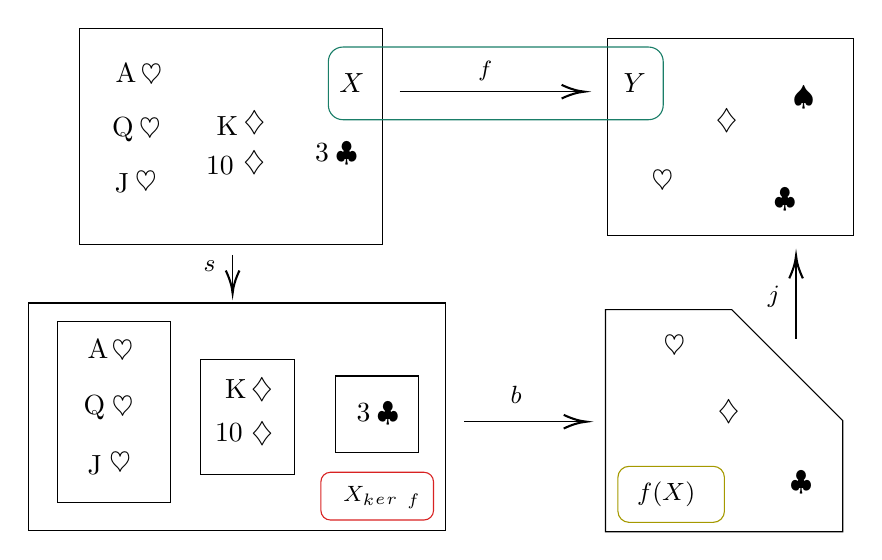
\begin{tikzpicture}[x=0.75pt,y=0.75pt,yscale=-1,xscale=1]
               %uncomment if require: \path (0,283); %set diagram left start at 0, and has height of 283

               %Shape: Rectangle [id:dp706505862263574] 
               \draw   (136.2,20.93) -- (281.87,20.93) -- (281.87,124.93) -- (136.2,124.93) -- cycle ;
               %Straight Lines [id:da3693556638631299] 
               \draw    (209.87,130.07) -- (209.87,146.6) ;
               \draw [shift={(209.87,148.6)}, rotate = 270] [color={rgb, 255:red, 0; green, 0; blue, 0 }  ][line width=0.75]    (10.93,-3.29) .. controls (6.95,-1.4) and (3.31,-0.3) .. (0,0) .. controls (3.31,0.3) and (6.95,1.4) .. (10.93,3.29)   ;
               %Shape: Rectangle [id:dp04842635536868545] 
               \draw   (111.4,153.33) -- (312.27,153.33) -- (312.27,262.87) -- (111.4,262.87) -- cycle ;
               %Shape: Rectangle [id:dp4296555353151592] 
               \draw   (125.6,162.07) -- (179.87,162.07) -- (179.87,249.27) -- (125.6,249.27) -- cycle ;
               %Shape: Rectangle [id:dp10721044735746443] 
               \draw   (194.4,180.47) -- (239.87,180.47) -- (239.87,236.07) -- (194.4,236.07) -- cycle ;
               %Shape: Rectangle [id:dp05111312242076149] 
               \draw   (259.6,188.47) -- (299.47,188.47) -- (299.47,225.27) -- (259.6,225.27) -- cycle ;
               %Rounded Rect [id:dp10074530866221898] 
               \draw  [color={rgb, 255:red, 216; green, 34; blue, 34 }  ,draw opacity=1 ] (252.4,239.47) .. controls (252.4,236.93) and (254.46,234.87) .. (257,234.87) -- (302.07,234.87) .. controls (304.61,234.87) and (306.67,236.93) .. (306.67,239.47) -- (306.67,253.27) .. controls (306.67,255.81) and (304.61,257.87) .. (302.07,257.87) -- (257,257.87) .. controls (254.46,257.87) and (252.4,255.81) .. (252.4,253.27) -- cycle ;
               %Straight Lines [id:da9478383111897926] 
               \draw    (321.5,210.5) -- (378.33,210.5) ;
               \draw [shift={(380.33,210.5)}, rotate = 180] [color={rgb, 255:red, 0; green, 0; blue, 0 }  ][line width=0.75]    (10.93,-3.29) .. controls (6.95,-1.4) and (3.31,-0.3) .. (0,0) .. controls (3.31,0.3) and (6.95,1.4) .. (10.93,3.29)   ;
               %Snip Single Corner Rect [id:dp578989805840413] 
               \draw   (389.5,156.5) -- (450.33,156.5) -- (503.83,210) -- (503.83,263.5) -- (389.5,263.5) -- cycle ;
               %Rounded Rect [id:dp27487588222286563] 
               \draw  [color={rgb, 255:red, 165; green, 153; blue, 0 }  ,draw opacity=1 ] (395.5,237.4) .. controls (395.5,234.42) and (397.92,232) .. (400.9,232) -- (441.43,232) .. controls (444.42,232) and (446.83,234.42) .. (446.83,237.4) -- (446.83,253.6) .. controls (446.83,256.58) and (444.42,259) .. (441.43,259) -- (400.9,259) .. controls (397.92,259) and (395.5,256.58) .. (395.5,253.6) -- cycle ;
               %Straight Lines [id:da08328439599003512] 
               \draw    (481.33,170.5) -- (481.33,132.5) ;
               \draw [shift={(481.33,130.5)}, rotate = 90] [color={rgb, 255:red, 0; green, 0; blue, 0 }  ][line width=0.75]    (10.93,-3.29) .. controls (6.95,-1.4) and (3.31,-0.3) .. (0,0) .. controls (3.31,0.3) and (6.95,1.4) .. (10.93,3.29)   ;
               %Shape: Rectangle [id:dp9272690052599577] 
               \draw   (390.5,26) -- (508.83,26) -- (508.83,121) -- (390.5,121) -- cycle ;
               %Rounded Rect [id:dp384981296655891] 
               \draw  [color={rgb, 255:red, 26; green, 126; blue, 104 }  ,draw opacity=1 ] (256,37) .. controls (256,33.13) and (259.13,30) .. (263,30) -- (410.33,30) .. controls (414.2,30) and (417.33,33.13) .. (417.33,37) -- (417.33,58) .. controls (417.33,61.87) and (414.2,65) .. (410.33,65) -- (263,65) .. controls (259.13,65) and (256,61.87) .. (256,58) -- cycle ;
               %Straight Lines [id:da6106767055811906] 
               \draw    (290.33,51.5) -- (377.33,51.5) ;
               \draw [shift={(379.33,51.5)}, rotate = 180] [color={rgb, 255:red, 0; green, 0; blue, 0 }  ][line width=0.75]    (10.93,-3.29) .. controls (6.95,-1.4) and (3.31,-0.3) .. (0,0) .. controls (3.31,0.3) and (6.95,1.4) .. (10.93,3.29)   ;
               \draw (151.93,89.87) node [anchor=north west][inner sep=0.75pt]   [align=left] {J};
               \draw (161.6,88.6) node [anchor=north west][inner sep=0.75pt]    {$\heartsuit $};
               \draw (150.6,62.53) node [anchor=north west][inner sep=0.75pt]   [align=left] {Q};
               \draw (163.6,62.93) node [anchor=north west][inner sep=0.75pt]    {$\heartsuit $};
               \draw (152.27,36.87) node [anchor=north west][inner sep=0.75pt]   [align=left] {A};
               \draw (164.27,37.27) node [anchor=north west][inner sep=0.75pt]    {$\heartsuit $};
               \draw (195.8,81.67) node [anchor=north west][inner sep=0.75pt]   [align=left] {10};
               \draw (213.8,79.07) node [anchor=north west][inner sep=0.75pt]    {$\diamondsuit $};
               \draw (200.87,62.4) node [anchor=north west][inner sep=0.75pt]   [align=left] {K};
               \draw (213.87,59.8) node [anchor=north west][inner sep=0.75pt]    {$\diamondsuit $};
               \draw (248.33,75.33) node [anchor=north west][inner sep=0.75pt]   [align=left] {3};
               \draw (258.33,74.73) node [anchor=north west][inner sep=0.75pt]    {$\clubsuit $};
               \draw (194.6,131.6) node [anchor=north west][inner sep=0.75pt]  [font=\small]  {$s$};
               \draw (138.75,225.36) node [anchor=north west][inner sep=0.75pt]   [align=left] {J};
               \draw (149.27,223.98) node [anchor=north west][inner sep=0.75pt]    {$\heartsuit $};
               \draw (136.86,196.57) node [anchor=north west][inner sep=0.75pt]   [align=left] {Q};
               \draw (150.4,196.95) node [anchor=north west][inner sep=0.75pt]    {$\heartsuit $};
               \draw (138.78,169.54) node [anchor=north west][inner sep=0.75pt]   [align=left] {A};
               \draw (150.32,169.91) node [anchor=north west][inner sep=0.75pt]    {$\heartsuit $};
               \draw (200.13,210.4) node [anchor=north west][inner sep=0.75pt]   [align=left] {10};
               \draw (217.63,209.62) node [anchor=north west][inner sep=0.75pt]    {$\diamondsuit $};
               \draw (205.04,189.06) node [anchor=north west][inner sep=0.75pt]   [align=left] {K};
               \draw (217.58,188.27) node [anchor=north west][inner sep=0.75pt]    {$\diamondsuit $};
               \draw (268.3,200.57) node [anchor=north west][inner sep=0.75pt]   [align=left] {3};
               \draw (278.28,199.84) node [anchor=north west][inner sep=0.75pt]    {$\clubsuit $};
               \draw (262,240.27) node [anchor=north west][inner sep=0.75pt]  [font=\footnotesize]  {$X_{k}{}_{e}{}_{r}{}_{\ }{}_{f}$};
               \draw (342.5,191.9) node [anchor=north west][inner sep=0.75pt]  [font=\small]  {$b$};
               \draw (416.27,167.77) node [anchor=north west][inner sep=0.75pt]    {$\heartsuit $};
               \draw (442.37,198.8) node [anchor=north west][inner sep=0.75pt]    {$\diamondsuit $};
               \draw (477.33,233.23) node [anchor=north west][inner sep=0.75pt]    {$\clubsuit $};
               \draw (403.5,238.4) node [anchor=north west][inner sep=0.75pt]  [font=\small]  {$f( X)$};
               \draw (466.5,143.9) node [anchor=north west][inner sep=0.75pt]  [font=\small]  {$j$};
               \draw (469.5,96.9) node [anchor=north west][inner sep=0.75pt]    {$\clubsuit $};
               \draw (441.5,58.9) node [anchor=north west][inner sep=0.75pt]    {$\diamondsuit $};
               \draw (410.5,87.9) node [anchor=north west][inner sep=0.75pt]    {$\heartsuit $};
               \draw (478.5,47.4) node [anchor=north west][inner sep=0.75pt]    {$\spadesuit $};
               \draw (397,41.4) node [anchor=north west][inner sep=0.75pt]    {$Y$};
               \draw (260,41.4) node [anchor=north west][inner sep=0.75pt]    {$X$};
               \draw (327,35.4) node [anchor=north west][inner sep=0.75pt]  [font=\footnotesize]  {$f$};
            \end{tikzpicture} 

            Ilustração do Primeiro Teorema de Isomorfismo.
         \end{center}
         O domínio $X$ é o conjunto das cartas em mãos. O contradomínio $Y$ é o conjunto completo de naipes. A função $f$ mapeia cada carta na mão para o seu naipe, portanto duas cartas estão na relação $ker\ f$ se e somente se eles estão no mesmo naipe. A classe de equivalência $$ \left[Q\heartsuit\right]_{ker\ f} = \left\{J\heartsuit , Q\heartsuit , A\heartsuit \right\}$$ consiste de todas as copas na mão, a classe $$\left[K\diamondsuit \right]_{ker\ f} = \left\{10\diamondsuit , K\diamondsuit \right\}$$ consiste de todos os ouros na mão, e a classe $\left[3\clubsuit \right]_{ker\ f}$ contém o único de paus na mão. A imagem $$f(X) = \left\{\heartsuit , \diamondsuit , \clubsuit  \right\}$$ é conjunto dos naipes que estão na mão. O primeiro teorema de isomorfismo exibe esse conjunto como isomórfico ao conjunto $$X_{ker\ f} = \left\{\left[Q\heartsuit\right]_{ker\ f}, \left[K\diamondsuit\right]_{ker\ f}, \left[3\clubsuit\right]_{ker\ f}\right\}$$ das classes de equivalência. De fato, ambos $f(X)$ e $X_{ker\ f}$ possuem 3 elementos cada. O fato de que os 3 elementos do conjunto $X_{ker\ f}$ são conjuntos é irrelevante. Quando estamos lidando com conjuntos de classes de equivalência desconsidere os detalhes internos das classes por um momento, e apenas considere cada classe como um elemento.

   \subsection{Aritmética Modular}
      Considere $a = dq + r$ ($0 \leq r < d$). Sendo $a$ o dividendo, $q$ o quociente, $d$ o divisor e o $r$ o resto.

      Para cada inteiro $a$, define-se $(a mod b)$ por
      \begin{equation}\label{MOD}
         a = qd + (a mod d).
      \end{equation}
      Logicamente $(a mod d)$ representa o resto. Agora considere a função
      \begin{equation}\label{MODFUNCTION}
         f: \Z \to \N;\quad a \mapsto a mod d.
      \end{equation}
      As classes de núcleo $[a]_{mod\ d}$ dessa função são conhecidas como \emph{classes de congruência módulo d}. Dois inteiros $a$ e $d$ são ditos serem \emph{congruentes módulo} $d$, denotado por
      \begin{equation}\label{AMODB}
         a \equiv b\quad mod\ d,
      \end{equation}
      se eles estão relacionado pela relação de núcleo $ker\ f$, ou (equivalentemente) se eles estão na mesma classe de congruência, ou se eles deixam o mesmo resto após a divisão por $d$. Para facilitar o uso de \ref{AMODB} será util resumir mais formas equivalentes da relação.
      \begin{stat}[Caracterização de Congruência]
         Seja $d$ um inteiro positivo. Para inteiros $a$ e $b$, são equivalentes:
         \begin{enumerate}[(a)]
            \item $a\equiv b\quad mod\ b$;
            \item $d \mid a - b$;
            \item $a-b$ é um múltiplo de $d$.
         \end{enumerate}
      \end{stat}
      A bijeção $b$ do primeiro teorema de isomorfismo para conjuntos provê um isomorfismo
      \begin{alignat}{2}
         &\ \Z_{mod\ d} \to \dfrac{\Z}{d}\nonumber\\
         &[a]_{mod\ d} \mapsto\ a\ mod\ d.
         \nonumber
      \end{alignat}
      entre o conjunto das classes de congruência módulo $d$ e o conjunto $$\dfrac{\Z}{d} = \{0,1,2,... , d-1\}$$ dos restos ou inteiros módulo $d$, a imagem da função \ref{MODFUNCTION}. O isomorfismo é frequentemente usado para identificar uma classe de congruência com seu resto representativo, assim o conjunto das classes de congruência é então escrito como $\dfrac{\Z}{d}$.

      Para $d=2$ o conjunto $\dfrac{\Z}{2} = \{0,1\}$ consiste de \emph{dois bits} ou \emph{digitos binários} $0$ e $1$.

      \begin{stat}
         Seja $d$ um inteiro positivo. Suponha que para inteiros $a_{i}$ e $b_{i}$ ($i = 1,2$), $$a_{1} \equiv b_{1}\ \ mod\ d\quad \&\quad a_{2} \equiv b_{2}\ \ mod\ d.$$ Então $$a_{1} + a_{2} \equiv b_{1} + b_{2}\ \ mod\ d\quad \&\quad a_{1}\cdot a_{2} \equiv b_{1} \cdot b_{2}\ \ mod\ d.$$
      \end{stat}
      \begin{corollary}
         Existem operações \emph{bem definidas}
         \begin{equation}\label{ADITTOP}
            [a]_{mod\ d} + [b]_{mod\ d} = [a+b]_{mod\ d}
         \end{equation}
         e
         \begin{equation}
            [a]_{mod\ d} \cdot [b]_{mod\ d} = [a\cdot b]_{mod\ d}
         \end{equation}
         nos conjuntos $\Z_{mod\ d}$ e $\dfrac{\Z}{d}$.
      \end{corollary}
      Note que para cada elemento $a$ de $\dfrac{\Z}{d}$, a função $$\dfrac{\Z}{d} \to \dfrac{\Z}{d};\ x\mapsto a+x$$
      é a permutação $$\left((0\ mod\ d)\ (1\ mod\ d)\ (2\ mod\ d)\ ...\ (-1\ mod\ d)\right)^{a}$$ do grupo cíclico $C_{d}$.
\newpage



%%%%%%%%%%%%%%%%%%%%%%%%%%%%%%%%%%%%%%%%%%%%%%%%%%%%%%%%%%%%%%%%%%%%%%%%%%%%%%
%%%%%%%%%%%%%%%%%%%%%%%%%%%%%%%%%%%%%%%%%%%%%%%%%%%%%%%%%%%%%%%%%%%%%%%%%%%%%%
%%%%%%%%%%%%%%%%%%%%%%%%%%%%%%%%%%%%%%%%%%%%%%%%%%%%%%%%%%%%%%%%%%%%%%%%%%%%%%
%%%%%%%%%%%%%%%%%%%%%%%%%%%%%%%%%%%%%%%%%%%%%%%%%%%%%%%%%%%%%%%%%%%%%%%%%%%%%%
%%%%%%%%%%%%%%%%%%%%%%%%%%%%%%%%%%%%%%%%%%%%%%%%%%%%%%%%%%%%%%%%%%%%%%%%%%%%%%
%%%%%%%%%%%%%%%%%%%%%%%%%%%%%%%%%%%%%%%%%%%%%%%%%%%%%%%%%%%%%%%%%%%%%%%%%%%%%%
%%%%%%%%%%%%%%%%%%%%%%%%%%%%%%%%%%%%%%%%%%%%%%%%%%%%%%%%%%%%%%%%%%%%%%%%%%%%%%
%%%%%%%%%%%%%%%%%%%%%%%%%%%%%%%%%%%%%%%%%%%%%%%%%%%%%%%%%%%%%%%%%%%%%%%%%%%%%%
%%%%%%%%%%%%%%%%%%%%%%%%%%%%%%%%%%%%%%%%%%%%%%%%%%%%%%%%%%%%%%%%%%%%%%%%%%%%%%
%%%%%%%%%%%%%%%%%%%%%%%%%%%%%%%%%%%%%%%%%%%%%%%%%%%%%%%%%%%%%%%%%%%%%%%%%%%%%%
%%%%%%%%%%%%%%%%%%%%%%%%%%%%%%%%%%%%%%%%%%%%%%%%%%%%%%%%%%%%%%%%%%%%%%%%%%%%%%